\documentclass[tikz,border=4pt]{standalone}
\usepackage[T1]{fontenc}
\usepackage{helvet}
\renewcommand{\familydefault}{\sfdefault}
\usepackage{amsmath,amssymb}
\usetikzlibrary{arrows.meta,positioning,fit,calc,backgrounds}
\definecolor{ink}{HTML}{1F1F1E}
\definecolor{muted}{HTML}{6B6A63}
\definecolor{line}{HTML}{8A8980}
\definecolor{fillA}{HTML}{EEF4FC}
\definecolor{fillB}{HTML}{F6F5F1}
\definecolor{accent2}{HTML}{C4501F}
\begin{document}
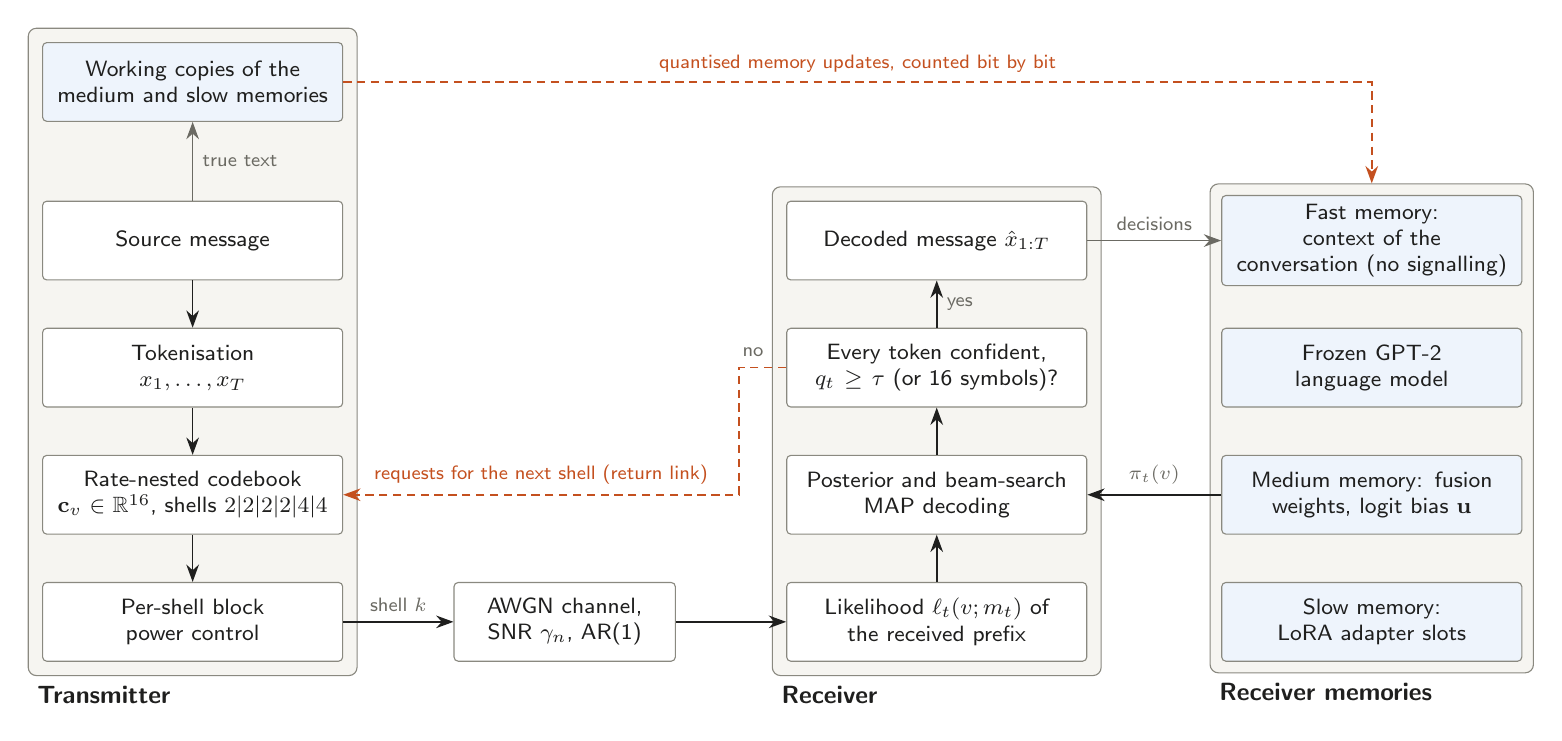
\begin{tikzpicture}[
  font=\footnotesize, text=ink,
  >={Stealth[length=2.2mm,width=1.6mm]},
  box/.style={draw=line, fill=white, rounded corners=1.5pt, align=center, minimum height=10mm, inner sep=3pt, text width=36mm},
  mem/.style={draw=line, fill=fillA, rounded corners=1.5pt, align=center, minimum height=10mm, inner sep=3pt, text width=36mm},
  flow/.style={->, draw=ink, line width=0.6pt},
  ctrl/.style={->, draw=accent2, line width=0.6pt, dash pattern=on 3pt off 2pt},
  note/.style={font=\scriptsize, text=muted, align=center}
]
% ---------------- receiver column (built first: it sets the rows)
\node[box] (lik) {Likelihood $\ell_t(v;m_t)$ of\\ the received prefix};
\node[box, above=6mm of lik] (post) {Posterior and beam-search\\ MAP decoding};
\node[box, above=6mm of post] (conf) {Every token confident,\\ $q_t\ge\tau$ (or 16 symbols)?};
\node[box, above=6mm of conf] (out) {Decoded message $\hat{x}_{1:T}$};
\draw[flow] (lik) -- (post);
\draw[flow] (post) -- (conf);
\draw[flow] (conf) -- node[note, right]{yes} (out);

% receiver memories, row-aligned with the receiver column
\node[mem, right=17mm of out] (ctx) {Fast memory: context of the\\ conversation (no signalling)};
\node[mem, right=17mm of conf] (prior) {Frozen GPT-2\\ language model};
\node[mem, right=17mm of post] (bias) {Medium memory: fusion\\ weights, logit bias $\mathbf{u}$};
\node[mem, right=17mm of lik] (lora) {Slow memory:\\ LoRA adapter slots};
\begin{scope}[on background layer]
\node[draw=line, fill=fillB, rounded corners=3pt, inner sep=4pt, fit=(ctx)(prior)(bias)(lora)] (memfit) {};
\end{scope}
\draw[flow, draw=muted] (out.east) -- node[note, above]{decisions} (ctx.west);
\draw[flow] (bias.west) -- node[note, above]{$\pi_t(v)$} (post.east);

% ---------------- channel and transmitter (left of the receiver)
\node[box, text width=26mm, left=14mm of lik] (ch) {AWGN channel,\\ SNR $\gamma_n$, AR(1)};
\node[box, left=14mm of ch] (pc) {Per-shell block\\ power control};
\node[box, above=6mm of pc] (cb) {Rate-nested codebook\\ $\mathbf{c}_v\in\mathbb{R}^{16}$, shells $2|2|2|2|4|4$};
\node[box, above=6mm of cb] (tok) {Tokenisation\\ $x_1,\dots,x_T$};
\node[box, above=6mm of tok] (src) {Source message};
\draw[flow] (src) -- (tok);
\draw[flow] (tok) -- (cb);
\draw[flow] (cb) -- (pc);
\draw[flow] (pc) -- node[note, above]{shell $k$} (ch);
\draw[flow] (ch) -- (lik);
\node[mem, above=10mm of src] (txmem) {Working copies of the\\ medium and slow memories};
\draw[flow, draw=muted] (src.north) -- node[note, right]{true text} (txmem.south);

% ---------------- return link: requests for the next shell
\node[note, anchor=south] at ($(conf.west)+(-4.2mm,0.2mm)$) {no};
\draw[ctrl] (conf.west) -- ($(conf.west)+(-6mm,0)$) |- node[note, pos=0.75, above, text=accent2]{requests for the next shell (return link)} ($(cb.east)+(0,0)$);

% ---------------- synchronisation of the shipped memories
\draw[ctrl] (txmem.east) -- node[note, above, text=accent2]{quantised memory updates, counted bit by bit} (txmem.east -| memfit.north) -- (memfit.north);

% ---------------- groups
\begin{scope}[on background layer]
\node[draw=line, fill=fillB, rounded corners=3pt, inner sep=5pt, fit=(txmem)(src)(tok)(cb)(pc)] (tx) {};
\node[draw=line, fill=fillB, rounded corners=3pt, inner sep=5pt, fit=(lik)(post)(conf)(out)] (rx) {};
\end{scope}
\node[font=\small\bfseries, anchor=north west] at (tx.south west) {Transmitter};
\node[font=\small\bfseries, anchor=north west] at (rx.south west) {Receiver};
\node[font=\small\bfseries, anchor=north west] at (memfit.south west) {Receiver memories};
\end{tikzpicture}
\end{document}
